\documentclass[1p]{elsarticle_modified}
%\bibliographystyle{elsarticle-num}

%\usepackage[colorlinks]{hyperref}
%\usepackage{abbrmath_seonhwa} %\Abb, \Ascr, \Acal ,\Abf, \Afrak
\usepackage{amsfonts}
\usepackage{amssymb}
\usepackage{amsmath}
\usepackage{amsthm}
\usepackage{scalefnt}
\usepackage{amsbsy}
\usepackage{kotex}
\usepackage{caption}
\usepackage{subfig}
\usepackage{color}
\usepackage{graphicx}
\usepackage{xcolor} %% white, black, red, green, blue, cyan, magenta, yellow
\usepackage{float}
\usepackage{setspace}
\usepackage{hyperref}

\usepackage{tikz}
\usetikzlibrary{arrows}

\usepackage{multirow}
\usepackage{array} % fixed length table
\usepackage{hhline}

%%%%%%%%%%%%%%%%%%%%%
\makeatletter
\renewcommand*\env@matrix[1][\arraystretch]{%
	\edef\arraystretch{#1}%
	\hskip -\arraycolsep
	\let\@ifnextchar\new@ifnextchar
	\array{*\c@MaxMatrixCols c}}
\makeatother %https://tex.stackexchange.com/questions/14071/how-can-i-increase-the-line-spacing-in-a-matrix
%%%%%%%%%%%%%%%

\usepackage[normalem]{ulem}

\newcommand{\msout}[1]{\ifmmode\text{\sout{\ensuremath{#1}}}\else\sout{#1}\fi}
%SOURCE: \msout is \stkout macro in https://tex.stackexchange.com/questions/20609/strikeout-in-math-mode

\newcommand{\cancel}[1]{
	\ifmmode
	{\color{red}\msout{#1}}
	\else
	{\color{red}\sout{#1}}
	\fi
}

\newcommand{\add}[1]{
	{\color{blue}\uwave{#1}}
}

\newcommand{\replace}[2]{
	\ifmmode
	{\color{red}\msout{#1}}{\color{blue}\uwave{#2}}
	\else
	{\color{red}\sout{#1}}{\color{blue}\uwave{#2}}
	\fi
}

\newcommand{\Sol}{\mathcal{S}} %segment
\newcommand{\D}{D} %diagram
\newcommand{\A}{\mathcal{A}} %arc


%%%%%%%%%%%%%%%%%%%%%%%%%%%%%5 test

\def\sl{\operatorname{\textup{SL}}(2,\Cbb)}
\def\psl{\operatorname{\textup{PSL}}(2,\Cbb)}
\def\quan{\mkern 1mu \triangleright \mkern 1mu}

\theoremstyle{definition}
\newtheorem{thm}{Theorem}[section]
\newtheorem{prop}[thm]{Proposition}
\newtheorem{lem}[thm]{Lemma}
\newtheorem{ques}[thm]{Question}
\newtheorem{cor}[thm]{Corollary}
\newtheorem{defn}[thm]{Definition}
\newtheorem{exam}[thm]{Example}
\newtheorem{rmk}[thm]{Remark}
\newtheorem{alg}[thm]{Algorithm}

\newcommand{\I}{\sqrt{-1}}
\begin{document}

%\begin{frontmatter}
%
%\title{Boundary parabolic representations of knots up to 8 crossings}
%
%%% Group authors per affiliation:
%\author{Yunhi Cho} 
%\address{Department of Mathematics, University of Seoul, Seoul, Korea}
%\ead{yhcho@uos.ac.kr}
%
%
%\author{Seonhwa Kim} %\fnref{s_kim}}
%\address{Center for Geometry and Physics, Institute for Basic Science, Pohang, 37673, Korea}
%\ead{ryeona17@ibs.re.kr}
%
%\author{Hyuk Kim}
%\address{Department of Mathematical Sciences, Seoul National University, Seoul 08826, Korea}
%\ead{hyukkim@snu.ac.kr}
%
%\author{Seokbeom Yoon}
%\address{Department of Mathematical Sciences, Seoul National University, Seoul, 08826,  Korea}
%\ead{sbyoon15@snu.ac.kr}
%
%\begin{abstract}
%We find all boundary parabolic representation of knots up to 8 crossings.
%
%\end{abstract}
%\begin{keyword}
%    \MSC[2010] 57M25 
%\end{keyword}
%
%\end{frontmatter}

%\linenumbers
%\tableofcontents
%
\newcommand\colored[1]{\textcolor{white}{\rule[-0.35ex]{0.8em}{1.4ex}}\kern-0.8em\color{red} #1}%
%\newcommand\colored[1]{\textcolor{white}{ #1}\kern-2.17ex	\textcolor{white}{ #1}\kern-1.81ex	\textcolor{white}{ #1}\kern-2.15ex\color{red}#1	}

{\Large $\underline{12a_{0882}~(K12a_{0882})}$}

\setlength{\tabcolsep}{10pt}
\renewcommand{\arraystretch}{1.6}
\vspace{1cm}\begin{tabular}{m{100pt}>{\centering\arraybackslash}m{274pt}}
\multirow{5}{120pt}{
	\centering
	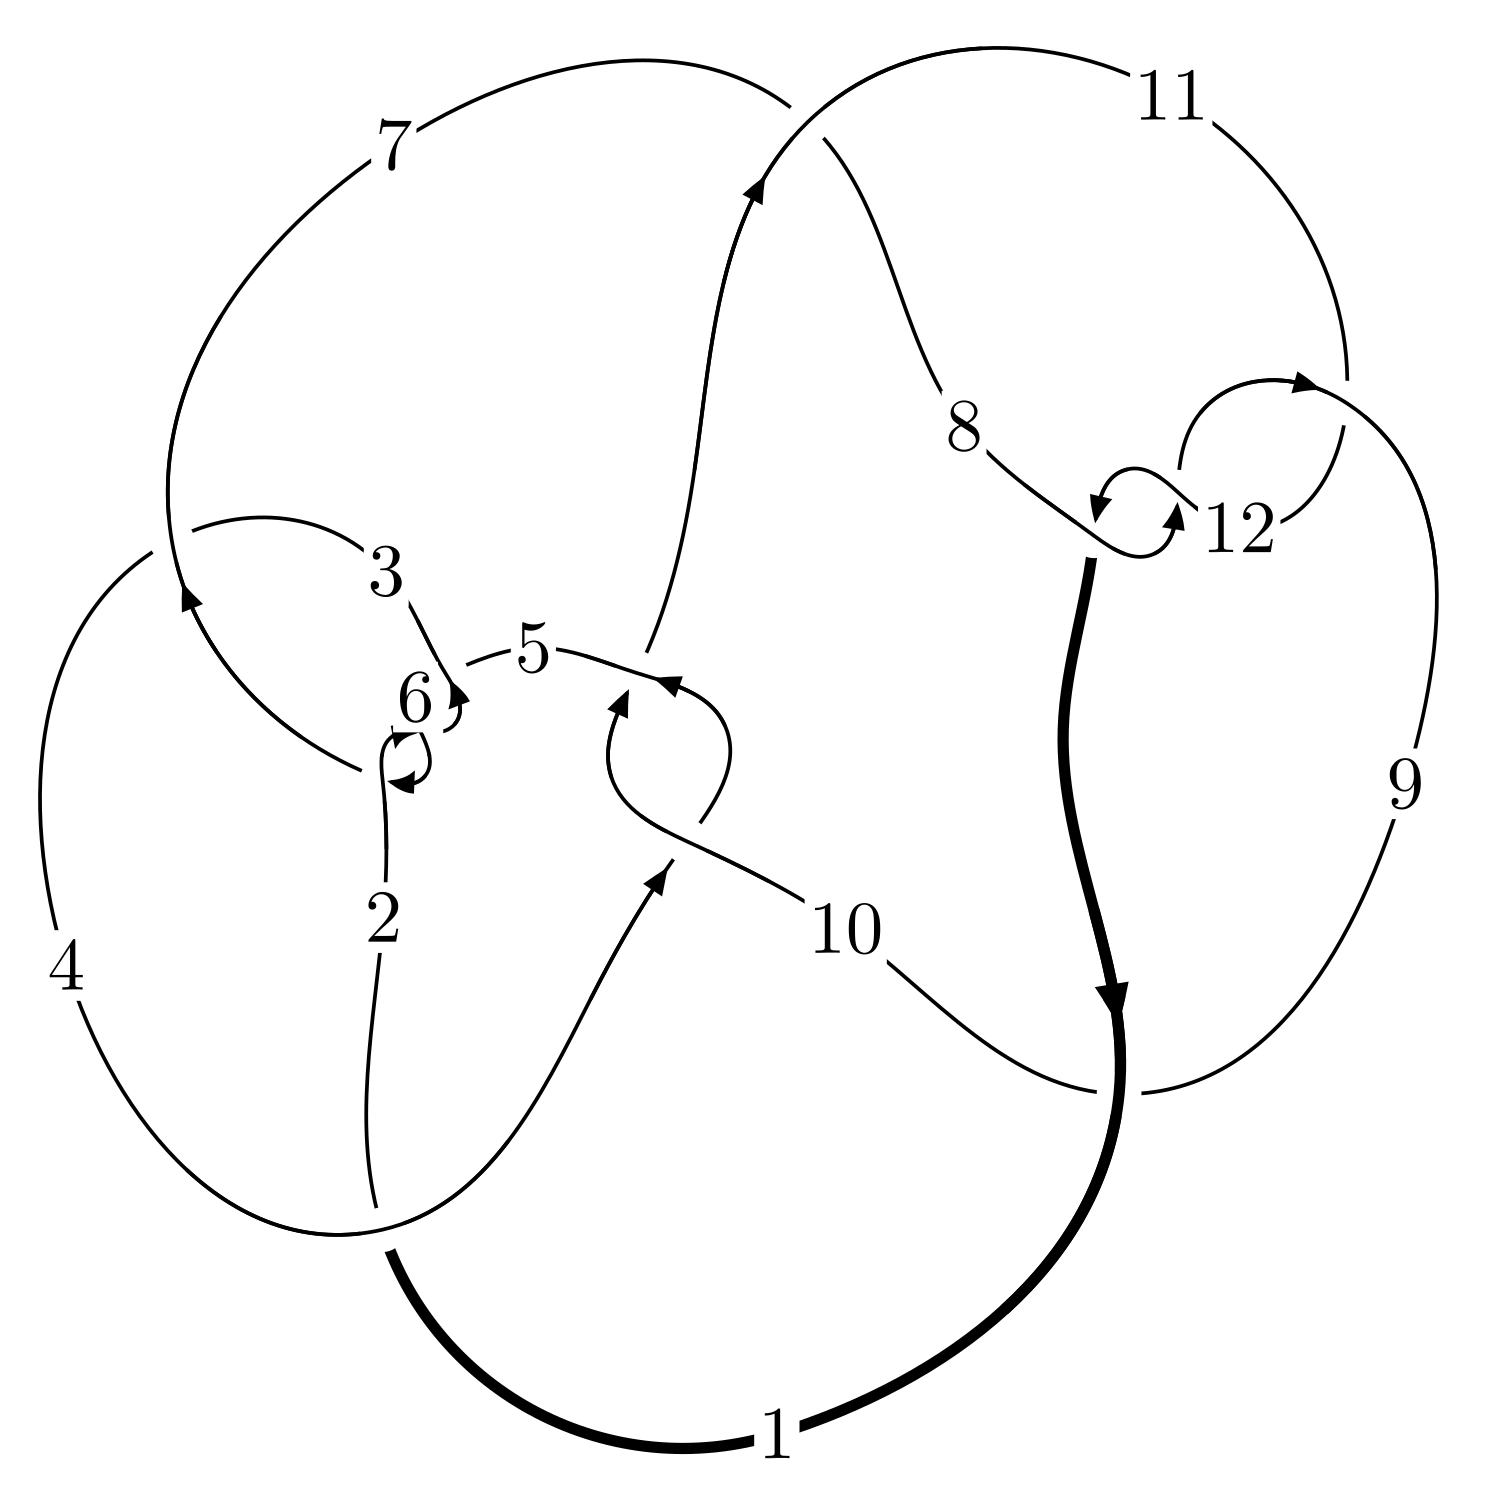
\includegraphics[width=112pt]{../../../GIT/diagram.site/Diagrams/png/1683_12a_0882.png}\\
\ \ \ A knot diagram\footnotemark}&
\allowdisplaybreaks
\textbf{Linearized knot diagam} \\
\cline{2-2}
 &
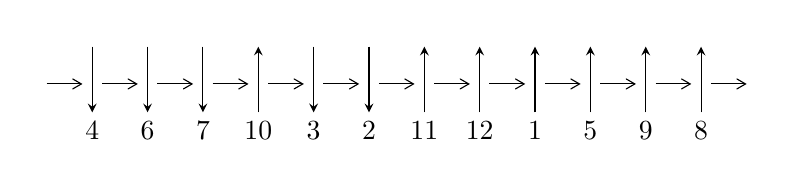
\begin{tikzpicture}[x=20pt, y=17pt]
	% nodes
	\node (C0) at (0, 0) {};
	\node (C1) at (1, 0) {};
	\node (C1U) at (1, +1) {};
	\node (C1D) at (1, -1) {4};

	\node (C2) at (2, 0) {};
	\node (C2U) at (2, +1) {};
	\node (C2D) at (2, -1) {6};

	\node (C3) at (3, 0) {};
	\node (C3U) at (3, +1) {};
	\node (C3D) at (3, -1) {7};

	\node (C4) at (4, 0) {};
	\node (C4U) at (4, +1) {};
	\node (C4D) at (4, -1) {10};

	\node (C5) at (5, 0) {};
	\node (C5U) at (5, +1) {};
	\node (C5D) at (5, -1) {3};

	\node (C6) at (6, 0) {};
	\node (C6U) at (6, +1) {};
	\node (C6D) at (6, -1) {2};

	\node (C7) at (7, 0) {};
	\node (C7U) at (7, +1) {};
	\node (C7D) at (7, -1) {11};

	\node (C8) at (8, 0) {};
	\node (C8U) at (8, +1) {};
	\node (C8D) at (8, -1) {12};

	\node (C9) at (9, 0) {};
	\node (C9U) at (9, +1) {};
	\node (C9D) at (9, -1) {1};

	\node (C10) at (10, 0) {};
	\node (C10U) at (10, +1) {};
	\node (C10D) at (10, -1) {5};

	\node (C11) at (11, 0) {};
	\node (C11U) at (11, +1) {};
	\node (C11D) at (11, -1) {9};

	\node (C12) at (12, 0) {};
	\node (C12U) at (12, +1) {};
	\node (C12D) at (12, -1) {8};
	\node (C13) at (13, 0) {};

	% arrows
	\draw[->,>={angle 60}]
	(C0) edge (C1) (C1) edge (C2) (C2) edge (C3) (C3) edge (C4) (C4) edge (C5) (C5) edge (C6) (C6) edge (C7) (C7) edge (C8) (C8) edge (C9) (C9) edge (C10) (C10) edge (C11) (C11) edge (C12) (C12) edge (C13) ;	\draw[->,>=stealth]
	(C1U) edge (C1D) (C2U) edge (C2D) (C3U) edge (C3D) (C4D) edge (C4U) (C5U) edge (C5D) (C6U) edge (C6D) (C7D) edge (C7U) (C8D) edge (C8U) (C9D) edge (C9U) (C10D) edge (C10U) (C11D) edge (C11U) (C12D) edge (C12U) ;
	\end{tikzpicture} \\
\hhline{~~} \\& 
\textbf{Solving Sequence} \\ \cline{2-2} 
 &
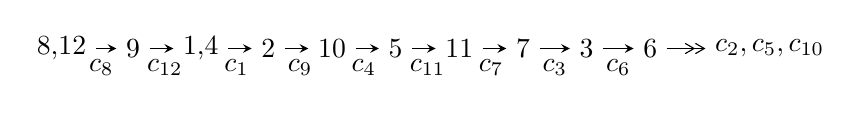
\begin{tikzpicture}[x=23pt, y=7pt]
	% node
	\node (A0) at (-1/8, 0) {8,12};
	\node (A1) at (1, 0) {9};
	\node (A2) at (33/16, 0) {1,4};
	\node (A3) at (25/8, 0) {2};
	\node (A4) at (33/8, 0) {10};
	\node (A5) at (41/8, 0) {5};
	\node (A6) at (49/8, 0) {11};
	\node (A7) at (57/8, 0) {7};
	\node (A8) at (65/8, 0) {3};
	\node (A9) at (73/8, 0) {6};
	\node (C1) at (1/2, -1) {$c_{8}$};
	\node (C2) at (3/2, -1) {$c_{12}$};
	\node (C3) at (21/8, -1) {$c_{1}$};
	\node (C4) at (29/8, -1) {$c_{9}$};
	\node (C5) at (37/8, -1) {$c_{4}$};
	\node (C6) at (45/8, -1) {$c_{11}$};
	\node (C7) at (53/8, -1) {$c_{7}$};
	\node (C8) at (61/8, -1) {$c_{3}$};
	\node (C9) at (69/8, -1) {$c_{6}$};
	\node (A10) at (11, 0) {$c_{2},c_{5},c_{10}$};

	% edge
	\draw[->,>=stealth]	
	(A0) edge (A1) (A1) edge (A2) (A2) edge (A3) (A3) edge (A4) (A4) edge (A5) (A5) edge (A6) (A6) edge (A7) (A7) edge (A8) (A8) edge (A9) ;
	\draw[->>,>={angle 60}]	
	(A9) edge (A10);
\end{tikzpicture} \\ 

\end{tabular} \\

\footnotetext{
The image of knot diagram is generated by the software ``\textbf{Draw programme}" developed by Andrew Bartholomew(\url{http://www.layer8.co.uk/maths/draw/index.htm\#Running-draw}), where we modified some parts for our purpose(\url{https://github.com/CATsTAILs/LinksPainter}).
}\phantom \\ \newline 
\centering \textbf{Ideals for irreducible components\footnotemark of $X_{\text{par}}$} 
 
\begin{align*}
I^u_{1}&=\langle 
4 u^{74}-16 u^{73}+\cdots+4 b-5,\;- u^{74}+8 u^{73}+\cdots+4 a+13,\;u^{75}-4 u^{74}+\cdots-6 u+1\rangle \\
I^u_{2}&=\langle 
u^2 a+b+a,\;u^2 a+a^2+u^2+a+u+1,\;u^3+u^2+2 u+1\rangle \\
I^u_{3}&=\langle 
- u^3+b- u,\;a+u,\;u^7+3 u^5+2 u^3- u-1\rangle \\
I^u_{4}&=\langle 
u^2+b+u+1,\;a+u,\;u^3+u^2+2 u+1\rangle \\
\\
\end{align*}
\raggedright * 4 irreducible components of $\dim_{\mathbb{C}}=0$, with total 91 representations.\\
\footnotetext{All coefficients of polynomials are rational numbers. But the coefficients are sometimes approximated in decimal forms when there is not enough margin.}
\newpage
\renewcommand{\arraystretch}{1}
\centering \section*{I. $I^u_{1}= \langle 4 u^{74}-16 u^{73}+\cdots+4 b-5,\;- u^{74}+8 u^{73}+\cdots+4 a+13,\;u^{75}-4 u^{74}+\cdots-6 u+1 \rangle$}
\flushleft \textbf{(i) Arc colorings}\\
\begin{tabular}{m{7pt} m{180pt} m{7pt} m{180pt} }
\flushright $a_{8}=$&$\begin{pmatrix}1\\0\end{pmatrix}$ \\
\flushright $a_{12}=$&$\begin{pmatrix}0\\u\end{pmatrix}$ \\
\flushright $a_{9}=$&$\begin{pmatrix}1\\- u^2\end{pmatrix}$ \\
\flushright $a_{1}=$&$\begin{pmatrix}u\\u\end{pmatrix}$ \\
\flushright $a_{4}=$&$\begin{pmatrix}\frac{1}{4} u^{74}-2 u^{73}+\cdots+\frac{65}{4} u-\frac{13}{4}\\- u^{74}+4 u^{73}+\cdots-4 u+\frac{5}{4}\end{pmatrix}$ \\
\flushright $a_{2}=$&$\begin{pmatrix}\frac{1}{4} u^{74}-\frac{3}{4} u^{73}+\cdots+7 u+\frac{3}{4}\\-\frac{1}{4} u^{74}+u^{73}+\cdots-\frac{9}{4} u+\frac{1}{2}\end{pmatrix}$ \\
\flushright $a_{10}=$&$\begin{pmatrix}- u^4- u^2+1\\- u^4-2 u^2\end{pmatrix}$ \\
\flushright $a_{5}=$&$\begin{pmatrix}\frac{15}{4} u^{74}-10 u^{73}+\cdots+\frac{23}{4} u-\frac{3}{4}\\2 u^{74}- u^{73}+\cdots-8 u+\frac{7}{4}\end{pmatrix}$ \\
\flushright $a_{11}=$&$\begin{pmatrix}- u\\u^3+u\end{pmatrix}$ \\
\flushright $a_{7}=$&$\begin{pmatrix}- u^4- u^2+1\\u^6+2 u^4+u^2\end{pmatrix}$ \\
\flushright $a_{3}=$&$\begin{pmatrix}\frac{13}{4} u^{74}-\frac{55}{4} u^{73}+\cdots+\frac{53}{2} u-\frac{17}{4}\\u^{74}-\frac{15}{4} u^{73}+\cdots-\frac{11}{4} u+\frac{5}{4}\end{pmatrix}$ \\
\flushright $a_{6}=$&$\begin{pmatrix}- u^{74}+\frac{19}{4} u^{73}+\cdots-\frac{7}{4} u+\frac{3}{4}\\-\frac{3}{4} u^{74}+3 u^{73}+\cdots+\frac{9}{4} u-\frac{1}{2}\end{pmatrix}$\\&\end{tabular}
\flushleft \textbf{(ii) Obstruction class $= -1$}\\~\\
\flushleft \textbf{(iii) Cusp Shapes $= -\frac{9}{2} u^{74}+\frac{19}{2} u^{73}+\cdots-\frac{39}{2} u-\frac{9}{4}$}\\~\\
\newpage\renewcommand{\arraystretch}{1}
\flushleft \textbf{(iv) u-Polynomials at the component}\newline \\
\begin{tabular}{m{50pt}|m{274pt}}
Crossings & \hspace{64pt}u-Polynomials at each crossing \\
\hline $$\begin{aligned}c_{1}\end{aligned}$$&$\begin{aligned}
&u^{75}-14 u^{74}+\cdots+204 u+801
\end{aligned}$\\
\hline $$\begin{aligned}c_{2},c_{5},c_{6}\end{aligned}$$&$\begin{aligned}
&u^{75}-4 u^{74}+\cdots+10 u-1
\end{aligned}$\\
\hline $$\begin{aligned}c_{3}\end{aligned}$$&$\begin{aligned}
&u^{75}+4 u^{74}+\cdots+2274 u-153
\end{aligned}$\\
\hline $$\begin{aligned}c_{4},c_{10}\end{aligned}$$&$\begin{aligned}
&u^{75}+6 u^{74}+\cdots-3072 u-512
\end{aligned}$\\
\hline $$\begin{aligned}c_{7},c_{9}\end{aligned}$$&$\begin{aligned}
&u^{75}-4 u^{74}+\cdots-750 u-153
\end{aligned}$\\
\hline $$\begin{aligned}c_{8},c_{11},c_{12}\end{aligned}$$&$\begin{aligned}
&u^{75}+4 u^{74}+\cdots-6 u-1
\end{aligned}$\\
\hline
\end{tabular}\\~\\
\newpage\renewcommand{\arraystretch}{1}
\flushleft \textbf{(v) Riley Polynomials at the component}\newline \\
\begin{tabular}{m{50pt}|m{274pt}}
Crossings & \hspace{64pt}Riley Polynomials at each crossing \\
\hline $$\begin{aligned}c_{1}\end{aligned}$$&$\begin{aligned}
&y^{75}+42 y^{74}+\cdots+136940526 y-641601
\end{aligned}$\\
\hline $$\begin{aligned}c_{2},c_{5},c_{6}\end{aligned}$$&$\begin{aligned}
&y^{75}+70 y^{74}+\cdots+34 y-1
\end{aligned}$\\
\hline $$\begin{aligned}c_{3}\end{aligned}$$&$\begin{aligned}
&y^{75}+14 y^{74}+\cdots+593622 y-23409
\end{aligned}$\\
\hline $$\begin{aligned}c_{4},c_{10}\end{aligned}$$&$\begin{aligned}
&y^{75}-42 y^{74}+\cdots+3276800 y-262144
\end{aligned}$\\
\hline $$\begin{aligned}c_{7},c_{9}\end{aligned}$$&$\begin{aligned}
&y^{75}-58 y^{74}+\cdots-431082 y-23409
\end{aligned}$\\
\hline $$\begin{aligned}c_{8},c_{11},c_{12}\end{aligned}$$&$\begin{aligned}
&y^{75}+62 y^{74}+\cdots-14 y-1
\end{aligned}$\\
\hline
\end{tabular}\\~\\
\newpage\flushleft \textbf{(vi) Complex Volumes and Cusp Shapes}
$$\begin{array}{c|c|c}  
\text{Solutions to }I^u_{1}& \I (\text{vol} + \sqrt{-1}CS) & \text{Cusp shape}\\
 \hline 
\begin{aligned}
u &= -0.129331 + 1.117110 I \\
a &= \phantom{-}0.29237 - 1.85419 I \\
b &= \phantom{-}0.11903 - 1.46059 I\end{aligned}
 & \phantom{-}1.67101 - 2.28476 I & \phantom{-0.000000 } 0 \\ \hline\begin{aligned}
u &= -0.129331 - 1.117110 I \\
a &= \phantom{-}0.29237 + 1.85419 I \\
b &= \phantom{-}0.11903 + 1.46059 I\end{aligned}
 & \phantom{-}1.67101 + 2.28476 I & \phantom{-0.000000 } 0 \\ \hline\begin{aligned}
u &= \phantom{-}0.864283 + 0.073603 I \\
a &= -0.630215 - 0.318792 I \\
b &= -0.46463 - 1.50057 I\end{aligned}
 & \phantom{-}14.07080 + 0.97614 I & \phantom{-}11.89444 - 0.69772 I \\ \hline\begin{aligned}
u &= \phantom{-}0.864283 - 0.073603 I \\
a &= -0.630215 + 0.318792 I \\
b &= -0.46463 + 1.50057 I\end{aligned}
 & \phantom{-}14.07080 - 0.97614 I & \phantom{-}11.89444 + 0.69772 I \\ \hline\begin{aligned}
u &= \phantom{-}0.851962 + 0.130511 I \\
a &= \phantom{-}0.189706 + 0.407751 I \\
b &= -0.20536 + 2.41576 I\end{aligned}
 & \phantom{-}12.0915 + 11.1738 I & \phantom{-}9.92293 - 6.69276 I \\ \hline\begin{aligned}
u &= \phantom{-}0.851962 - 0.130511 I \\
a &= \phantom{-}0.189706 - 0.407751 I \\
b &= -0.20536 - 2.41576 I\end{aligned}
 & \phantom{-}12.0915 - 11.1738 I & \phantom{-}9.92293 + 6.69276 I \\ \hline\begin{aligned}
u &= \phantom{-}0.838542 + 0.118303 I \\
a &= -0.263667 - 0.275157 I \\
b &= \phantom{-}0.30731 - 2.10324 I\end{aligned}
 & \phantom{-}6.28260 + 7.50607 I & \phantom{-}6.31085 - 6.58507 I \\ \hline\begin{aligned}
u &= \phantom{-}0.838542 - 0.118303 I \\
a &= -0.263667 + 0.275157 I \\
b &= \phantom{-}0.30731 + 2.10324 I\end{aligned}
 & \phantom{-}6.28260 - 7.50607 I & \phantom{-}6.31085 + 6.58507 I \\ \hline\begin{aligned}
u &= \phantom{-}0.834761 + 0.091281 I \\
a &= \phantom{-}0.443254 + 0.200964 I \\
b &= -0.17545 + 1.64029 I\end{aligned}
 & \phantom{-}7.24740 + 3.22206 I & \phantom{-}8.45543 - 0.86065 I \\ \hline\begin{aligned}
u &= \phantom{-}0.834761 - 0.091281 I \\
a &= \phantom{-}0.443254 - 0.200964 I \\
b &= -0.17545 - 1.64029 I\end{aligned}
 & \phantom{-}7.24740 - 3.22206 I & \phantom{-}8.45543 + 0.86065 I\\
 \hline 
 \end{array}$$\newpage$$\begin{array}{c|c|c}  
\text{Solutions to }I^u_{1}& \I (\text{vol} + \sqrt{-1}CS) & \text{Cusp shape}\\
 \hline 
\begin{aligned}
u &= -0.806243 + 0.042985 I \\
a &= \phantom{-}0.254905 + 0.770452 I \\
b &= \phantom{-}0.64512 + 2.35548 I\end{aligned}
 & \phantom{-}8.28866 - 4.61277 I & \phantom{-}9.57496 + 3.37665 I \\ \hline\begin{aligned}
u &= -0.806243 - 0.042985 I \\
a &= \phantom{-}0.254905 - 0.770452 I \\
b &= \phantom{-}0.64512 - 2.35548 I\end{aligned}
 & \phantom{-}8.28866 + 4.61277 I & \phantom{-}9.57496 - 3.37665 I \\ \hline\begin{aligned}
u &= \phantom{-}0.417667 + 1.122760 I \\
a &= \phantom{-}2.24416 - 1.33147 I \\
b &= \phantom{-}0.82696 - 1.40165 I\end{aligned}
 & \phantom{-}9.05288 - 6.61172 I & \phantom{-0.000000 } 0 \\ \hline\begin{aligned}
u &= \phantom{-}0.417667 - 1.122760 I \\
a &= \phantom{-}2.24416 + 1.33147 I \\
b &= \phantom{-}0.82696 + 1.40165 I\end{aligned}
 & \phantom{-}9.05288 + 6.61172 I & \phantom{-0.000000 } 0 \\ \hline\begin{aligned}
u &= \phantom{-}0.394262 + 1.136570 I \\
a &= -1.88247 + 1.23446 I \\
b &= -0.590542 + 1.186780 I\end{aligned}
 & \phantom{-}3.16758 - 3.06037 I & \phantom{-0.000000 } 0 \\ \hline\begin{aligned}
u &= \phantom{-}0.394262 - 1.136570 I \\
a &= -1.88247 - 1.23446 I \\
b &= -0.590542 - 1.186780 I\end{aligned}
 & \phantom{-}3.16758 + 3.06037 I & \phantom{-0.000000 } 0 \\ \hline\begin{aligned}
u &= -0.767081 + 0.032918 I \\
a &= -0.147823 - 0.586406 I \\
b &= -0.41161 - 1.84908 I\end{aligned}
 & \phantom{-}2.54564 - 1.71234 I & \phantom{-}5.68970 + 3.98160 I \\ \hline\begin{aligned}
u &= -0.767081 - 0.032918 I \\
a &= -0.147823 + 0.586406 I \\
b &= -0.41161 + 1.84908 I\end{aligned}
 & \phantom{-}2.54564 + 1.71234 I & \phantom{-}5.68970 - 3.98160 I \\ \hline\begin{aligned}
u &= \phantom{-}0.387354 + 1.172960 I \\
a &= \phantom{-}1.54778 - 0.81015 I \\
b &= \phantom{-}0.496497 - 0.735271 I\end{aligned}
 & \phantom{-}3.93329 + 1.17961 I & \phantom{-0.000000 } 0 \\ \hline\begin{aligned}
u &= \phantom{-}0.387354 - 1.172960 I \\
a &= \phantom{-}1.54778 + 0.81015 I \\
b &= \phantom{-}0.496497 + 0.735271 I\end{aligned}
 & \phantom{-}3.93329 - 1.17961 I & \phantom{-0.000000 } 0\\
 \hline 
 \end{array}$$\newpage$$\begin{array}{c|c|c}  
\text{Solutions to }I^u_{1}& \I (\text{vol} + \sqrt{-1}CS) & \text{Cusp shape}\\
 \hline 
\begin{aligned}
u &= \phantom{-}0.761899 + 0.044601 I \\
a &= \phantom{-}0.670042 - 0.120108 I \\
b &= -1.140900 + 0.673722 I\end{aligned}
 & \phantom{-}5.34357 + 3.86193 I & \phantom{-}9.73760 - 4.61433 I \\ \hline\begin{aligned}
u &= \phantom{-}0.761899 - 0.044601 I \\
a &= \phantom{-}0.670042 + 0.120108 I \\
b &= -1.140900 - 0.673722 I\end{aligned}
 & \phantom{-}5.34357 - 3.86193 I & \phantom{-}9.73760 + 4.61433 I \\ \hline\begin{aligned}
u &= -0.502648 + 0.555980 I \\
a &= \phantom{-}1.35292 - 0.76273 I \\
b &= \phantom{-}0.424196 + 0.870841 I\end{aligned}
 & \phantom{-}6.99841 - 6.56505 I & \phantom{-}7.94758 + 6.80228 I \\ \hline\begin{aligned}
u &= -0.502648 - 0.555980 I \\
a &= \phantom{-}1.35292 + 0.76273 I \\
b &= \phantom{-}0.424196 - 0.870841 I\end{aligned}
 & \phantom{-}6.99841 + 6.56505 I & \phantom{-}7.94758 - 6.80228 I \\ \hline\begin{aligned}
u &= \phantom{-}0.417996 + 1.195510 I \\
a &= -1.81445 + 0.17291 I \\
b &= -0.943590 + 0.346371 I\end{aligned}
 & \phantom{-}10.62020 + 3.61647 I & \phantom{-0.000000 } 0 \\ \hline\begin{aligned}
u &= \phantom{-}0.417996 - 1.195510 I \\
a &= -1.81445 - 0.17291 I \\
b &= -0.943590 - 0.346371 I\end{aligned}
 & \phantom{-}10.62020 - 3.61647 I & \phantom{-0.000000 } 0 \\ \hline\begin{aligned}
u &= -0.586451 + 0.420780 I \\
a &= -0.745096 - 0.020246 I \\
b &= \phantom{-}0.568271 - 1.084970 I\end{aligned}
 & \phantom{-}7.43119 + 2.66733 I & \phantom{-}9.42694 + 0.01688 I \\ \hline\begin{aligned}
u &= -0.586451 - 0.420780 I \\
a &= -0.745096 + 0.020246 I \\
b &= \phantom{-}0.568271 + 1.084970 I\end{aligned}
 & \phantom{-}7.43119 - 2.66733 I & \phantom{-}9.42694 - 0.01688 I \\ \hline\begin{aligned}
u &= -0.352653 + 1.230150 I \\
a &= -2.08694 - 2.25380 I \\
b &= -1.15302 - 2.28427 I\end{aligned}
 & \phantom{-}4.63286 + 0.43633 I & \phantom{-0.000000 } 0 \\ \hline\begin{aligned}
u &= -0.352653 - 1.230150 I \\
a &= -2.08694 + 2.25380 I \\
b &= -1.15302 + 2.28427 I\end{aligned}
 & \phantom{-}4.63286 - 0.43633 I & \phantom{-0.000000 } 0\\
 \hline 
 \end{array}$$\newpage$$\begin{array}{c|c|c}  
\text{Solutions to }I^u_{1}& \I (\text{vol} + \sqrt{-1}CS) & \text{Cusp shape}\\
 \hline 
\begin{aligned}
u &= -0.316269 + 1.249700 I \\
a &= \phantom{-}1.82642 + 1.56645 I \\
b &= \phantom{-}1.16268 + 1.70863 I\end{aligned}
 & -1.20445 - 2.19229 I & \phantom{-0.000000 } 0 \\ \hline\begin{aligned}
u &= -0.316269 - 1.249700 I \\
a &= \phantom{-}1.82642 - 1.56645 I \\
b &= \phantom{-}1.16268 - 1.70863 I\end{aligned}
 & -1.20445 + 2.19229 I & \phantom{-0.000000 } 0 \\ \hline\begin{aligned}
u &= \phantom{-}0.053632 + 1.289800 I \\
a &= -1.55559 + 0.97168 I \\
b &= -0.72624 + 1.73649 I\end{aligned}
 & -0.99866 + 4.23513 I & \phantom{-0.000000 } 0 \\ \hline\begin{aligned}
u &= \phantom{-}0.053632 - 1.289800 I \\
a &= -1.55559 - 0.97168 I \\
b &= -0.72624 - 1.73649 I\end{aligned}
 & -0.99866 - 4.23513 I & \phantom{-0.000000 } 0 \\ \hline\begin{aligned}
u &= \phantom{-}0.016620 + 1.304390 I \\
a &= \phantom{-}1.194330 - 0.735726 I \\
b &= \phantom{-}0.69581 - 1.49341 I\end{aligned}
 & -5.82265 + 0.81095 I & \phantom{-0.000000 } 0 \\ \hline\begin{aligned}
u &= \phantom{-}0.016620 - 1.304390 I \\
a &= \phantom{-}1.194330 + 0.735726 I \\
b &= \phantom{-}0.69581 + 1.49341 I\end{aligned}
 & -5.82265 - 0.81095 I & \phantom{-0.000000 } 0 \\ \hline\begin{aligned}
u &= -0.667774 + 0.163365 I \\
a &= \phantom{-}0.235125 + 0.105097 I \\
b &= \phantom{-}1.132700 + 0.443466 I\end{aligned}
 & \phantom{-}4.25302 - 0.78723 I & \phantom{-}8.08019 + 0.69488 I \\ \hline\begin{aligned}
u &= -0.667774 - 0.163365 I \\
a &= \phantom{-}0.235125 - 0.105097 I \\
b &= \phantom{-}1.132700 - 0.443466 I\end{aligned}
 & \phantom{-}4.25302 + 0.78723 I & \phantom{-}8.08019 - 0.69488 I \\ \hline\begin{aligned}
u &= \phantom{-}0.321229 + 1.276340 I \\
a &= \phantom{-}0.975526 + 0.758046 I \\
b &= \phantom{-}1.38917 - 0.31193 I\end{aligned}
 & -2.32532 + 3.88876 I & \phantom{-0.000000 } 0 \\ \hline\begin{aligned}
u &= \phantom{-}0.321229 - 1.276340 I \\
a &= \phantom{-}0.975526 - 0.758046 I \\
b &= \phantom{-}1.38917 + 0.31193 I\end{aligned}
 & -2.32532 - 3.88876 I & \phantom{-0.000000 } 0\\
 \hline 
 \end{array}$$\newpage$$\begin{array}{c|c|c}  
\text{Solutions to }I^u_{1}& \I (\text{vol} + \sqrt{-1}CS) & \text{Cusp shape}\\
 \hline 
\begin{aligned}
u &= -0.099287 + 1.314930 I \\
a &= -0.318472 + 0.820675 I \\
b &= -0.439087 + 1.148180 I\end{aligned}
 & -3.46404 - 2.05434 I & \phantom{-0.000000 } 0 \\ \hline\begin{aligned}
u &= -0.099287 - 1.314930 I \\
a &= -0.318472 - 0.820675 I \\
b &= -0.439087 - 1.148180 I\end{aligned}
 & -3.46404 + 2.05434 I & \phantom{-0.000000 } 0 \\ \hline\begin{aligned}
u &= -0.450416 + 0.509884 I \\
a &= -0.960127 + 0.859309 I \\
b &= -0.166013 - 0.591858 I\end{aligned}
 & \phantom{-}1.28106 - 3.47044 I & \phantom{-}3.88375 + 7.68592 I \\ \hline\begin{aligned}
u &= -0.450416 - 0.509884 I \\
a &= -0.960127 - 0.859309 I \\
b &= -0.166013 + 0.591858 I\end{aligned}
 & \phantom{-}1.28106 + 3.47044 I & \phantom{-}3.88375 - 7.68592 I \\ \hline\begin{aligned}
u &= -0.332166 + 1.293110 I \\
a &= -2.54722 - 1.00893 I \\
b &= -1.85697 - 1.49469 I\end{aligned}
 & -1.59371 - 5.68239 I & \phantom{-0.000000 } 0 \\ \hline\begin{aligned}
u &= -0.332166 - 1.293110 I \\
a &= -2.54722 + 1.00893 I \\
b &= -1.85697 + 1.49469 I\end{aligned}
 & -1.59371 + 5.68239 I & \phantom{-0.000000 } 0 \\ \hline\begin{aligned}
u &= \phantom{-}0.331305 + 1.302290 I \\
a &= -1.56104 - 0.14984 I \\
b &= -1.55504 + 0.97937 I\end{aligned}
 & \phantom{-}1.12844 + 7.81474 I & \phantom{-0.000000 } 0 \\ \hline\begin{aligned}
u &= \phantom{-}0.331305 - 1.302290 I \\
a &= -1.56104 + 0.14984 I \\
b &= -1.55504 - 0.97937 I\end{aligned}
 & \phantom{-}1.12844 - 7.81474 I & \phantom{-0.000000 } 0 \\ \hline\begin{aligned}
u &= -0.355420 + 1.298670 I \\
a &= \phantom{-}3.07198 + 1.18787 I \\
b &= \phantom{-}2.20157 + 1.78185 I\end{aligned}
 & \phantom{-}4.10044 - 8.79609 I & \phantom{-0.000000 } 0 \\ \hline\begin{aligned}
u &= -0.355420 - 1.298670 I \\
a &= \phantom{-}3.07198 - 1.18787 I \\
b &= \phantom{-}2.20157 - 1.78185 I\end{aligned}
 & \phantom{-}4.10044 + 8.79609 I & \phantom{-0.000000 } 0\\
 \hline 
 \end{array}$$\newpage$$\begin{array}{c|c|c}  
\text{Solutions to }I^u_{1}& \I (\text{vol} + \sqrt{-1}CS) & \text{Cusp shape}\\
 \hline 
\begin{aligned}
u &= -0.036427 + 1.346260 I \\
a &= -0.607791 + 0.422715 I \\
b &= -0.629673 + 1.192930 I\end{aligned}
 & -3.35604 - 2.35859 I & \phantom{-0.000000 } 0 \\ \hline\begin{aligned}
u &= -0.036427 - 1.346260 I \\
a &= -0.607791 - 0.422715 I \\
b &= -0.629673 - 1.192930 I\end{aligned}
 & -3.35604 + 2.35859 I & \phantom{-0.000000 } 0 \\ \hline\begin{aligned}
u &= -0.204057 + 1.350880 I \\
a &= -0.508818 + 0.849448 I \\
b &= -0.815090 + 0.663922 I\end{aligned}
 & -3.59967 - 2.38098 I & \phantom{-0.000000 } 0 \\ \hline\begin{aligned}
u &= -0.204057 - 1.350880 I \\
a &= -0.508818 - 0.849448 I \\
b &= -0.815090 - 0.663922 I\end{aligned}
 & -3.59967 + 2.38098 I & \phantom{-0.000000 } 0 \\ \hline\begin{aligned}
u &= -0.269785 + 1.347060 I \\
a &= \phantom{-}1.64477 - 0.56880 I \\
b &= \phantom{-}1.62647 + 0.01247 I\end{aligned}
 & -0.50518 - 4.19710 I & \phantom{-0.000000 } 0 \\ \hline\begin{aligned}
u &= -0.269785 - 1.347060 I \\
a &= \phantom{-}1.64477 + 0.56880 I \\
b &= \phantom{-}1.62647 - 0.01247 I\end{aligned}
 & -0.50518 + 4.19710 I & \phantom{-0.000000 } 0 \\ \hline\begin{aligned}
u &= \phantom{-}0.391046 + 1.322010 I \\
a &= \phantom{-}1.06116 - 1.80811 I \\
b &= \phantom{-}0.48619 - 2.18356 I\end{aligned}
 & \phantom{-}9.70536 + 5.47983 I & \phantom{-0.000000 } 0 \\ \hline\begin{aligned}
u &= \phantom{-}0.391046 - 1.322010 I \\
a &= \phantom{-}1.06116 + 1.80811 I \\
b &= \phantom{-}0.48619 + 2.18356 I\end{aligned}
 & \phantom{-}9.70536 - 5.47983 I & \phantom{-0.000000 } 0 \\ \hline\begin{aligned}
u &= \phantom{-}0.368532 + 1.330510 I \\
a &= -1.73222 + 1.34594 I \\
b &= -1.12286 + 2.08477 I\end{aligned}
 & \phantom{-}2.78873 + 7.54981 I & \phantom{-0.000000 } 0 \\ \hline\begin{aligned}
u &= \phantom{-}0.368532 - 1.330510 I \\
a &= -1.73222 - 1.34594 I \\
b &= -1.12286 - 2.08477 I\end{aligned}
 & \phantom{-}2.78873 - 7.54981 I & \phantom{-0.000000 } 0\\
 \hline 
 \end{array}$$\newpage$$\begin{array}{c|c|c}  
\text{Solutions to }I^u_{1}& \I (\text{vol} + \sqrt{-1}CS) & \text{Cusp shape}\\
 \hline 
\begin{aligned}
u &= \phantom{-}0.368054 + 1.347150 I \\
a &= \phantom{-}2.22544 - 1.63294 I \\
b &= \phantom{-}1.36977 - 2.45177 I\end{aligned}
 & \phantom{-}1.67578 + 11.84830 I & \phantom{-0.000000 } 0 \\ \hline\begin{aligned}
u &= \phantom{-}0.368054 - 1.347150 I \\
a &= \phantom{-}2.22544 + 1.63294 I \\
b &= \phantom{-}1.36977 + 2.45177 I\end{aligned}
 & \phantom{-}1.67578 - 11.84830 I & \phantom{-0.000000 } 0 \\ \hline\begin{aligned}
u &= -0.103421 + 1.398990 I \\
a &= -0.156439 - 0.588353 I \\
b &= \phantom{-}0.497683 - 1.119190 I\end{aligned}
 & -4.75437 - 5.19853 I & \phantom{-0.000000 } 0 \\ \hline\begin{aligned}
u &= -0.103421 - 1.398990 I \\
a &= -0.156439 + 0.588353 I \\
b &= \phantom{-}0.497683 + 1.119190 I\end{aligned}
 & -4.75437 + 5.19853 I & \phantom{-0.000000 } 0 \\ \hline\begin{aligned}
u &= \phantom{-}0.373793 + 1.356110 I \\
a &= -2.39427 + 1.96966 I \\
b &= -1.37738 + 2.74063 I\end{aligned}
 & \phantom{-}7.4137 + 15.5822 I & \phantom{-0.000000 } 0 \\ \hline\begin{aligned}
u &= \phantom{-}0.373793 - 1.356110 I \\
a &= -2.39427 - 1.96966 I \\
b &= -1.37738 - 2.74063 I\end{aligned}
 & \phantom{-}7.4137 - 15.5822 I & \phantom{-0.000000 } 0 \\ \hline\begin{aligned}
u &= -0.11241 + 1.42300 I \\
a &= \phantom{-}0.455015 + 0.662998 I \\
b &= -0.434609 + 1.177910 I\end{aligned}
 & \phantom{-}0.66003 - 8.48529 I & \phantom{-0.000000 } 0 \\ \hline\begin{aligned}
u &= -0.11241 - 1.42300 I \\
a &= \phantom{-}0.455015 - 0.662998 I \\
b &= -0.434609 - 1.177910 I\end{aligned}
 & \phantom{-}0.66003 + 8.48529 I & \phantom{-0.000000 } 0 \\ \hline\begin{aligned}
u &= -0.484381\phantom{ +0.000000I} \\
a &= -0.253063\phantom{ +0.000000I} \\
b &= -0.395089\phantom{ +0.000000I}\end{aligned}
 & \phantom{-}0.828246\phantom{ +0.000000I} & \phantom{-}12.7290\phantom{ +0.000000I} \\ \hline\begin{aligned}
u &= -0.040668 + 0.478942 I \\
a &= \phantom{-}0.06428 - 2.03562 I \\
b &= -0.380831 - 0.239183 I\end{aligned}
 & \phantom{-}2.10140 - 1.97255 I & \phantom{-}1.62971 + 4.07824 I\\
 \hline 
 \end{array}$$\newpage$$\begin{array}{c|c|c}  
\text{Solutions to }I^u_{1}& \I (\text{vol} + \sqrt{-1}CS) & \text{Cusp shape}\\
 \hline 
\begin{aligned}
u &= -0.040668 - 0.478942 I \\
a &= \phantom{-}0.06428 + 2.03562 I \\
b &= -0.380831 + 0.239183 I\end{aligned}
 & \phantom{-}2.10140 + 1.97255 I & \phantom{-}1.62971 - 4.07824 I \\ \hline\begin{aligned}
u &= \phantom{-}0.268652 + 0.175360 I \\
a &= -0.22486 - 2.74712 I \\
b &= -0.722155 + 0.751154 I\end{aligned}
 & \phantom{-}3.41208 + 3.23701 I & -0.51319 - 4.60923 I \\ \hline\begin{aligned}
u &= \phantom{-}0.268652 - 0.175360 I \\
a &= -0.22486 + 2.74712 I \\
b &= -0.722155 - 0.751154 I\end{aligned}
 & \phantom{-}3.41208 - 3.23701 I & -0.51319 + 4.60923 I \\ \hline\begin{aligned}
u &= \phantom{-}0.113105 + 0.236302 I \\
a &= \phantom{-}0.51485 + 2.54920 I \\
b &= \phantom{-}0.559155 - 0.256506 I\end{aligned}
 & -1.187190 + 0.455593 I & -6.24430 - 1.84121 I \\ \hline\begin{aligned}
u &= \phantom{-}0.113105 - 0.236302 I \\
a &= \phantom{-}0.51485 - 2.54920 I \\
b &= \phantom{-}0.559155 + 0.256506 I\end{aligned}
 & -1.187190 - 0.455593 I & -6.24430 + 1.84121 I\\
 \hline 
 \end{array}$$\newpage\newpage\renewcommand{\arraystretch}{1}
\centering \section*{II. $I^u_{2}= \langle u^2 a+b+a,\;u^2 a+a^2+u^2+a+u+1,\;u^3+u^2+2 u+1 \rangle$}
\flushleft \textbf{(i) Arc colorings}\\
\begin{tabular}{m{7pt} m{180pt} m{7pt} m{180pt} }
\flushright $a_{8}=$&$\begin{pmatrix}1\\0\end{pmatrix}$ \\
\flushright $a_{12}=$&$\begin{pmatrix}0\\u\end{pmatrix}$ \\
\flushright $a_{9}=$&$\begin{pmatrix}1\\- u^2\end{pmatrix}$ \\
\flushright $a_{1}=$&$\begin{pmatrix}u\\u\end{pmatrix}$ \\
\flushright $a_{4}=$&$\begin{pmatrix}a\\- u^2 a- a\end{pmatrix}$ \\
\flushright $a_{2}=$&$\begin{pmatrix}- u^2 a- a u-2 a+u-1\\u^2 a+u^2+2 a+u+1\end{pmatrix}$ \\
\flushright $a_{10}=$&$\begin{pmatrix}- u\\- u^2- u-1\end{pmatrix}$ \\
\flushright $a_{5}=$&$\begin{pmatrix}a\\- u^2 a- a\end{pmatrix}$ \\
\flushright $a_{11}=$&$\begin{pmatrix}- u\\- u^2- u-1\end{pmatrix}$ \\
\flushright $a_{7}=$&$\begin{pmatrix}- u\\- u\end{pmatrix}$ \\
\flushright $a_{3}=$&$\begin{pmatrix}- u^2 a- a u\\-2 u^2 a- a u-2 a\end{pmatrix}$ \\
\flushright $a_{6}=$&$\begin{pmatrix}- a u- u-1\\u^2 a+2 u^2+2 a+3\end{pmatrix}$\\&\end{tabular}
\flushleft \textbf{(ii) Obstruction class $= 1$}\\~\\
\flushleft \textbf{(iii) Cusp Shapes $= -3 u^2 a+5 u^2- a+5 u+8$}\\~\\
\newpage\renewcommand{\arraystretch}{1}
\flushleft \textbf{(iv) u-Polynomials at the component}\newline \\
\begin{tabular}{m{50pt}|m{274pt}}
Crossings & \hspace{64pt}u-Polynomials at each crossing \\
\hline $$\begin{aligned}c_{1},c_{3}\end{aligned}$$&$\begin{aligned}
&(u^3+u^2-1)^2
\end{aligned}$\\
\hline $$\begin{aligned}c_{2},c_{11},c_{12}\end{aligned}$$&$\begin{aligned}
&(u^3- u^2+2 u-1)^2
\end{aligned}$\\
\hline $$\begin{aligned}c_{4},c_{10}\end{aligned}$$&$\begin{aligned}
&u^6
\end{aligned}$\\
\hline $$\begin{aligned}c_{5},c_{6},c_{8}\end{aligned}$$&$\begin{aligned}
&(u^3+u^2+2 u+1)^2
\end{aligned}$\\
\hline $$\begin{aligned}c_{7},c_{9}\end{aligned}$$&$\begin{aligned}
&(u^3- u^2+1)^2
\end{aligned}$\\
\hline
\end{tabular}\\~\\
\newpage\renewcommand{\arraystretch}{1}
\flushleft \textbf{(v) Riley Polynomials at the component}\newline \\
\begin{tabular}{m{50pt}|m{274pt}}
Crossings & \hspace{64pt}Riley Polynomials at each crossing \\
\hline $$\begin{aligned}c_{1},c_{3},c_{7}\\c_{9}\end{aligned}$$&$\begin{aligned}
&(y^3- y^2+2 y-1)^2
\end{aligned}$\\
\hline $$\begin{aligned}c_{2},c_{5},c_{6}\\c_{8},c_{11},c_{12}\end{aligned}$$&$\begin{aligned}
&(y^3+3 y^2+2 y-1)^2
\end{aligned}$\\
\hline $$\begin{aligned}c_{4},c_{10}\end{aligned}$$&$\begin{aligned}
&y^6
\end{aligned}$\\
\hline
\end{tabular}\\~\\
\newpage\flushleft \textbf{(vi) Complex Volumes and Cusp Shapes}
$$\begin{array}{c|c|c}  
\text{Solutions to }I^u_{2}& \I (\text{vol} + \sqrt{-1}CS) & \text{Cusp shape}\\
 \hline 
\begin{aligned}
u &= -0.215080 + 1.307140 I \\
a &= -0.662359 + 0.562280 I \\
b &= -0.754878\phantom{ +0.000000I}\end{aligned}
 & -4.13758 - 2.82812 I & -4.97655 + 4.84887 I \\ \hline\begin{aligned}
u &= -0.215080 + 1.307140 I \\
a &= \phantom{-}1.32472\phantom{ +0.000000I} \\
b &= \phantom{-}0.877439 + 0.744862 I\end{aligned}
 & \phantom{-0.000000 } -5.65624 I & \phantom{-}3.89456 + 5.95889 I \\ \hline\begin{aligned}
u &= -0.215080 - 1.307140 I \\
a &= -0.662359 - 0.562280 I \\
b &= -0.754878\phantom{ +0.000000I}\end{aligned}
 & -4.13758 + 2.82812 I & -4.97655 - 4.84887 I \\ \hline\begin{aligned}
u &= -0.215080 - 1.307140 I \\
a &= \phantom{-}1.32472\phantom{ +0.000000I} \\
b &= \phantom{-}0.877439 - 0.744862 I\end{aligned}
 & \phantom{-0.000000 -}5.65624 I & \phantom{-}3.89456 - 5.95889 I \\ \hline\begin{aligned}
u &= -0.569840\phantom{ +0.000000I} \\
a &= -0.662359 + 0.562280 I \\
b &= \phantom{-}0.877439 - 0.744862 I\end{aligned}
 & \phantom{-}4.13758 + 2.82812 I & \phantom{-}8.08199 - 1.11003 I \\ \hline\begin{aligned}
u &= -0.569840\phantom{ +0.000000I} \\
a &= -0.662359 - 0.562280 I \\
b &= \phantom{-}0.877439 + 0.744862 I\end{aligned}
 & \phantom{-}4.13758 - 2.82812 I & \phantom{-}8.08199 + 1.11003 I\\
 \hline 
 \end{array}$$\newpage\newpage\renewcommand{\arraystretch}{1}
\centering \section*{III. $I^u_{3}= \langle - u^3+b- u,\;a+u,\;u^7+3 u^5+2 u^3- u-1 \rangle$}
\flushleft \textbf{(i) Arc colorings}\\
\begin{tabular}{m{7pt} m{180pt} m{7pt} m{180pt} }
\flushright $a_{8}=$&$\begin{pmatrix}1\\0\end{pmatrix}$ \\
\flushright $a_{12}=$&$\begin{pmatrix}0\\u\end{pmatrix}$ \\
\flushright $a_{9}=$&$\begin{pmatrix}1\\- u^2\end{pmatrix}$ \\
\flushright $a_{1}=$&$\begin{pmatrix}u\\u\end{pmatrix}$ \\
\flushright $a_{4}=$&$\begin{pmatrix}- u\\u^3+u\end{pmatrix}$ \\
\flushright $a_{2}=$&$\begin{pmatrix}- u^5-2 u^3+u\\2 u+1\end{pmatrix}$ \\
\flushright $a_{10}=$&$\begin{pmatrix}- u^4- u^2+1\\- u^4-2 u^2\end{pmatrix}$ \\
\flushright $a_{5}=$&$\begin{pmatrix}u^4+u^2- u-1\\u^4+u^3+2 u^2+u\end{pmatrix}$ \\
\flushright $a_{11}=$&$\begin{pmatrix}- u\\u^3+u\end{pmatrix}$ \\
\flushright $a_{7}=$&$\begin{pmatrix}- u^4- u^2+1\\u^6+2 u^4+u^2\end{pmatrix}$ \\
\flushright $a_{3}=$&$\begin{pmatrix}u^5+2 u^3- u-1\\u^5+3 u^3+u^2+u\end{pmatrix}$ \\
\flushright $a_{6}=$&$\begin{pmatrix}u^6+u^4-2 u^2+1\\u^6+2 u^4- u^2- u\end{pmatrix}$\\&\end{tabular}
\flushleft \textbf{(ii) Obstruction class $= -1$}\\~\\
\flushleft \textbf{(iii) Cusp Shapes $= 6$}\\~\\
\newpage\renewcommand{\arraystretch}{1}
\flushleft \textbf{(iv) u-Polynomials at the component}\newline \\
\begin{tabular}{m{50pt}|m{274pt}}
Crossings & \hspace{64pt}u-Polynomials at each crossing \\
\hline $$\begin{aligned}c_{1}\end{aligned}$$&$\begin{aligned}
&u^7-2 u^6+u^5+2 u^4-4 u^3+6 u^2-3 u+3
\end{aligned}$\\
\hline $$\begin{aligned}c_{2},c_{5},c_{6}\\c_{8},c_{11},c_{12}\end{aligned}$$&$\begin{aligned}
&u^7+3 u^5+2 u^3- u+1
\end{aligned}$\\
\hline $$\begin{aligned}c_{3},c_{7},c_{9}\end{aligned}$$&$\begin{aligned}
&u^7- u^5-2 u^4+2 u^3+2 u^2-3 u+2
\end{aligned}$\\
\hline $$\begin{aligned}c_{4},c_{10}\end{aligned}$$&$\begin{aligned}
&(u-1)^7
\end{aligned}$\\
\hline
\end{tabular}\\~\\
\newpage\renewcommand{\arraystretch}{1}
\flushleft \textbf{(v) Riley Polynomials at the component}\newline \\
\begin{tabular}{m{50pt}|m{274pt}}
Crossings & \hspace{64pt}Riley Polynomials at each crossing \\
\hline $$\begin{aligned}c_{1}\end{aligned}$$&$\begin{aligned}
&y^7-2 y^6+y^5+6 y^4-2 y^3-24 y^2-27 y-9
\end{aligned}$\\
\hline $$\begin{aligned}c_{2},c_{5},c_{6}\\c_{8},c_{11},c_{12}\end{aligned}$$&$\begin{aligned}
&y^7+6 y^6+13 y^5+10 y^4-2 y^3-4 y^2+y-1
\end{aligned}$\\
\hline $$\begin{aligned}c_{3},c_{7},c_{9}\end{aligned}$$&$\begin{aligned}
&y^7-2 y^6+5 y^5-14 y^4+18 y^3-8 y^2+y-4
\end{aligned}$\\
\hline $$\begin{aligned}c_{4},c_{10}\end{aligned}$$&$\begin{aligned}
&(y-1)^7
\end{aligned}$\\
\hline
\end{tabular}\\~\\
\newpage\flushleft \textbf{(vi) Complex Volumes and Cusp Shapes}
$$\begin{array}{c|c|c}  
\text{Solutions to }I^u_{3}& \I (\text{vol} + \sqrt{-1}CS) & \text{Cusp shape}\\
 \hline 
\begin{aligned}
u &= \phantom{-}0.757137\phantom{ +0.000000I} \\
a &= -0.757137\phantom{ +0.000000I} \\
b &= \phantom{-}1.19117\phantom{ +0.000000I}\end{aligned}
 & \phantom{-}1.64493\phantom{ +0.000000I} & \phantom{-}6.00000\phantom{ +0.000000I} \\ \hline\begin{aligned}
u &= \phantom{-}0.311114 + 1.246820 I \\
a &= -0.311114 - 1.246820 I \\
b &= -1.109710 - 0.329390 I\end{aligned}
 & \phantom{-}1.64493\phantom{ +0.000000I} & \phantom{-}6.00000\phantom{ +0.000000I} \\ \hline\begin{aligned}
u &= \phantom{-}0.311114 - 1.246820 I \\
a &= -0.311114 + 1.246820 I \\
b &= -1.109710 + 0.329390 I\end{aligned}
 & \phantom{-}1.64493\phantom{ +0.000000I} & \phantom{-}6.00000\phantom{ +0.000000I} \\ \hline\begin{aligned}
u &= -0.501027 + 0.385135 I \\
a &= \phantom{-}0.501027 - 0.385135 I \\
b &= -0.403848 + 0.618048 I\end{aligned}
 & \phantom{-}1.64493\phantom{ +0.000000I} & \phantom{-}6.00000\phantom{ +0.000000I} \\ \hline\begin{aligned}
u &= -0.501027 - 0.385135 I \\
a &= \phantom{-}0.501027 + 0.385135 I \\
b &= -0.403848 - 0.618048 I\end{aligned}
 & \phantom{-}1.64493\phantom{ +0.000000I} & \phantom{-}6.00000\phantom{ +0.000000I} \\ \hline\begin{aligned}
u &= -0.18866 + 1.40255 I \\
a &= \phantom{-}0.18866 - 1.40255 I \\
b &= \phantom{-}0.91797 - 1.20672 I\end{aligned}
 & \phantom{-}1.64493\phantom{ +0.000000I} & \phantom{-}6.00000\phantom{ +0.000000I} \\ \hline\begin{aligned}
u &= -0.18866 - 1.40255 I \\
a &= \phantom{-}0.18866 + 1.40255 I \\
b &= \phantom{-}0.91797 + 1.20672 I\end{aligned}
 & \phantom{-}1.64493\phantom{ +0.000000I} & \phantom{-}6.00000\phantom{ +0.000000I}\\
 \hline 
 \end{array}$$\newpage\newpage\renewcommand{\arraystretch}{1}
\centering \section*{IV. $I^u_{4}= \langle u^2+b+u+1,\;a+u,\;u^3+u^2+2 u+1 \rangle$}
\flushleft \textbf{(i) Arc colorings}\\
\begin{tabular}{m{7pt} m{180pt} m{7pt} m{180pt} }
\flushright $a_{8}=$&$\begin{pmatrix}1\\0\end{pmatrix}$ \\
\flushright $a_{12}=$&$\begin{pmatrix}0\\u\end{pmatrix}$ \\
\flushright $a_{9}=$&$\begin{pmatrix}1\\- u^2\end{pmatrix}$ \\
\flushright $a_{1}=$&$\begin{pmatrix}u\\u\end{pmatrix}$ \\
\flushright $a_{4}=$&$\begin{pmatrix}- u\\- u^2- u-1\end{pmatrix}$ \\
\flushright $a_{2}=$&$\begin{pmatrix}2 u+1\\2 u\end{pmatrix}$ \\
\flushright $a_{10}=$&$\begin{pmatrix}- u\\- u^2- u-1\end{pmatrix}$ \\
\flushright $a_{5}=$&$\begin{pmatrix}- u\\- u^2- u-1\end{pmatrix}$ \\
\flushright $a_{11}=$&$\begin{pmatrix}- u\\- u^2- u-1\end{pmatrix}$ \\
\flushright $a_{7}=$&$\begin{pmatrix}- u\\- u\end{pmatrix}$ \\
\flushright $a_{3}=$&$\begin{pmatrix}-2 u-1\\- u^2-2 u-2\end{pmatrix}$ \\
\flushright $a_{6}=$&$\begin{pmatrix}-2 u^2-2 u\\-2 u^2- u\end{pmatrix}$\\&\end{tabular}
\flushleft \textbf{(ii) Obstruction class $= 1$}\\~\\
\flushleft \textbf{(iii) Cusp Shapes $= 0$}\\~\\
\newpage\renewcommand{\arraystretch}{1}
\flushleft \textbf{(iv) u-Polynomials at the component}\newline \\
\begin{tabular}{m{50pt}|m{274pt}}
Crossings & \hspace{64pt}u-Polynomials at each crossing \\
\hline $$\begin{aligned}c_{1},c_{3}\end{aligned}$$&$\begin{aligned}
&u^3+u^2-1
\end{aligned}$\\
\hline $$\begin{aligned}c_{2},c_{11},c_{12}\end{aligned}$$&$\begin{aligned}
&u^3- u^2+2 u-1
\end{aligned}$\\
\hline $$\begin{aligned}c_{4},c_{10}\end{aligned}$$&$\begin{aligned}
&u^3
\end{aligned}$\\
\hline $$\begin{aligned}c_{5},c_{6},c_{8}\end{aligned}$$&$\begin{aligned}
&u^3+u^2+2 u+1
\end{aligned}$\\
\hline $$\begin{aligned}c_{7},c_{9}\end{aligned}$$&$\begin{aligned}
&u^3- u^2+1
\end{aligned}$\\
\hline
\end{tabular}\\~\\
\newpage\renewcommand{\arraystretch}{1}
\flushleft \textbf{(v) Riley Polynomials at the component}\newline \\
\begin{tabular}{m{50pt}|m{274pt}}
Crossings & \hspace{64pt}Riley Polynomials at each crossing \\
\hline $$\begin{aligned}c_{1},c_{3},c_{7}\\c_{9}\end{aligned}$$&$\begin{aligned}
&y^3- y^2+2 y-1
\end{aligned}$\\
\hline $$\begin{aligned}c_{2},c_{5},c_{6}\\c_{8},c_{11},c_{12}\end{aligned}$$&$\begin{aligned}
&y^3+3 y^2+2 y-1
\end{aligned}$\\
\hline $$\begin{aligned}c_{4},c_{10}\end{aligned}$$&$\begin{aligned}
&y^3
\end{aligned}$\\
\hline
\end{tabular}\\~\\
\newpage\flushleft \textbf{(vi) Complex Volumes and Cusp Shapes}
$$\begin{array}{c|c|c}  
\text{Solutions to }I^u_{4}& \I (\text{vol} + \sqrt{-1}CS) & \text{Cusp shape}\\
 \hline 
\begin{aligned}
u &= -0.215080 + 1.307140 I \\
a &= \phantom{-}0.215080 - 1.307140 I \\
b &= \phantom{-}0.877439 - 0.744862 I\end{aligned}
 & \phantom{-0.000000 } 0 & \phantom{-0.000000 } 0 \\ \hline\begin{aligned}
u &= -0.215080 - 1.307140 I \\
a &= \phantom{-}0.215080 + 1.307140 I \\
b &= \phantom{-}0.877439 + 0.744862 I\end{aligned}
 & \phantom{-0.000000 } 0 & \phantom{-0.000000 } 0 \\ \hline\begin{aligned}
u &= -0.569840\phantom{ +0.000000I} \\
a &= \phantom{-}0.569840\phantom{ +0.000000I} \\
b &= -0.754878\phantom{ +0.000000I}\end{aligned}
 & \phantom{-0.000000 } 0 & \phantom{-0.000000 } 0\\
 \hline 
 \end{array}$$\newpage
\newpage\renewcommand{\arraystretch}{1}
\centering \section*{ V. u-Polynomials}
\begin{tabular}{m{50pt}|m{274pt}}
Crossings & \hspace{64pt}u-Polynomials at each crossing \\
\hline $$\begin{aligned}c_{1}\end{aligned}$$&$\begin{aligned}
&(u^3+u^2-1)^3(u^7-2 u^6+u^5+2 u^4-4 u^3+6 u^2-3 u+3)\\
&\cdot(u^{75}-14 u^{74}+\cdots+204 u+801)
\end{aligned}$\\
\hline $$\begin{aligned}c_{2}\end{aligned}$$&$\begin{aligned}
&((u^3- u^2+2 u-1)^3)(u^7+3 u^5+2 u^3- u+1)(u^{75}-4 u^{74}+\cdots+10 u-1)
\end{aligned}$\\
\hline $$\begin{aligned}c_{3}\end{aligned}$$&$\begin{aligned}
&(u^3+u^2-1)^3(u^7- u^5-2 u^4+2 u^3+2 u^2-3 u+2)\\
&\cdot(u^{75}+4 u^{74}+\cdots+2274 u-153)
\end{aligned}$\\
\hline $$\begin{aligned}c_{4},c_{10}\end{aligned}$$&$\begin{aligned}
&u^9(u-1)^7(u^{75}+6 u^{74}+\cdots-3072 u-512)
\end{aligned}$\\
\hline $$\begin{aligned}c_{5},c_{6}\end{aligned}$$&$\begin{aligned}
&((u^3+u^2+2 u+1)^3)(u^7+3 u^5+2 u^3- u+1)(u^{75}-4 u^{74}+\cdots+10 u-1)
\end{aligned}$\\
\hline $$\begin{aligned}c_{7},c_{9}\end{aligned}$$&$\begin{aligned}
&(u^3- u^2+1)^3(u^7- u^5-2 u^4+2 u^3+2 u^2-3 u+2)\\
&\cdot(u^{75}-4 u^{74}+\cdots-750 u-153)
\end{aligned}$\\
\hline $$\begin{aligned}c_{8}\end{aligned}$$&$\begin{aligned}
&((u^3+u^2+2 u+1)^3)(u^7+3 u^5+2 u^3- u+1)(u^{75}+4 u^{74}+\cdots-6 u-1)
\end{aligned}$\\
\hline $$\begin{aligned}c_{11},c_{12}\end{aligned}$$&$\begin{aligned}
&((u^3- u^2+2 u-1)^3)(u^7+3 u^5+2 u^3- u+1)(u^{75}+4 u^{74}+\cdots-6 u-1)
\end{aligned}$\\
\hline
\end{tabular}\newpage\renewcommand{\arraystretch}{1}
\centering \section*{ VI. Riley Polynomials}
\begin{tabular}{m{50pt}|m{274pt}}
Crossings & \hspace{64pt}Riley Polynomials at each crossing \\
\hline $$\begin{aligned}c_{1}\end{aligned}$$&$\begin{aligned}
&(y^3- y^2+2 y-1)^3(y^7-2 y^6+y^5+6 y^4-2 y^3-24 y^2-27 y-9)\\
&\cdot(y^{75}+42 y^{74}+\cdots+136940526 y-641601)
\end{aligned}$\\
\hline $$\begin{aligned}c_{2},c_{5},c_{6}\end{aligned}$$&$\begin{aligned}
&(y^3+3 y^2+2 y-1)^3(y^7+6 y^6+13 y^5+10 y^4-2 y^3-4 y^2+y-1)\\
&\cdot(y^{75}+70 y^{74}+\cdots+34 y-1)
\end{aligned}$\\
\hline $$\begin{aligned}c_{3}\end{aligned}$$&$\begin{aligned}
&(y^3- y^2+2 y-1)^3(y^7-2 y^6+5 y^5-14 y^4+18 y^3-8 y^2+y-4)\\
&\cdot(y^{75}+14 y^{74}+\cdots+593622 y-23409)
\end{aligned}$\\
\hline $$\begin{aligned}c_{4},c_{10}\end{aligned}$$&$\begin{aligned}
&y^9(y-1)^7(y^{75}-42 y^{74}+\cdots+3276800 y-262144)
\end{aligned}$\\
\hline $$\begin{aligned}c_{7},c_{9}\end{aligned}$$&$\begin{aligned}
&(y^3- y^2+2 y-1)^3(y^7-2 y^6+5 y^5-14 y^4+18 y^3-8 y^2+y-4)\\
&\cdot(y^{75}-58 y^{74}+\cdots-431082 y-23409)
\end{aligned}$\\
\hline $$\begin{aligned}c_{8},c_{11},c_{12}\end{aligned}$$&$\begin{aligned}
&(y^3+3 y^2+2 y-1)^3(y^7+6 y^6+13 y^5+10 y^4-2 y^3-4 y^2+y-1)\\
&\cdot(y^{75}+62 y^{74}+\cdots-14 y-1)
\end{aligned}$\\
\hline
\end{tabular}
\vskip 2pc
\end{document}